\documentclass[tikz,border=4pt]{standalone}
\usepackage{amsmath,amssymb}
\usetikzlibrary{positioning,arrows.meta,calc,fit,backgrounds}
\definecolor{qcol}{HTML}{EB6834}   % query genes
\definecolor{ycol}{HTML}{2A78D6}   % gene set
\definecolor{bcol}{HTML}{7A4E9E}   % overlap
\definecolor{gcol}{HTML}{B9B8B2}
\begin{document}
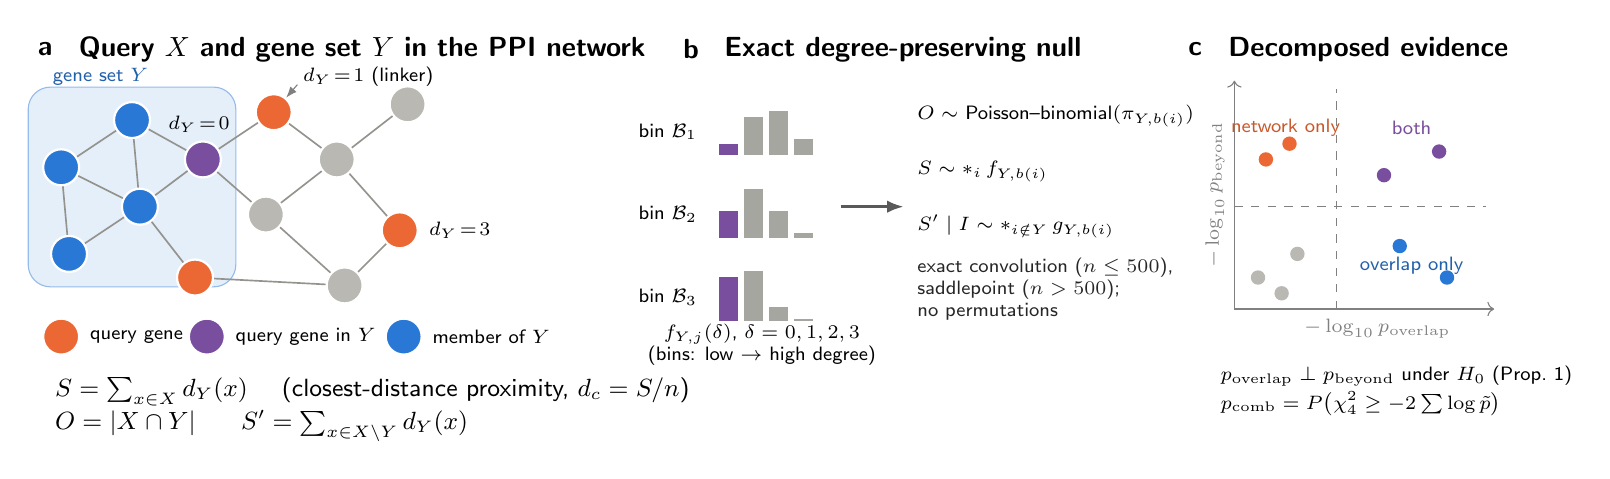
\begin{tikzpicture}[
  font=\sffamily\small,
  n/.style={circle,draw=white,line width=0.8pt,minimum size=13pt,inner sep=0pt,fill=gcol},
  qn/.style={n,fill=qcol}, yn/.style={n,fill=ycol}, bn/.style={n,fill=bcol},
  e/.style={gcol!80!black,line width=0.6pt},
  box/.style={draw=gray!50,rounded corners=4pt,inner sep=6pt},
  lab/.style={font=\sffamily\bfseries\normalsize},
  arr/.style={-{Latex[length=6pt]},line width=1pt,gray!70!black}]

% ---------------------------------------------------------------- (a) network
\begin{scope}
\node[lab] at (-0.2,3.3) {a};
\node[font=\sffamily\bfseries,anchor=west] at (0.1,3.3) {Query $X$ and gene set $Y$ in the PPI network};
\node[yn] (y1) at (0,1.8) {}; \node[yn] (y2) at (0.9,2.4) {}; \node[yn] (y3) at (1.0,1.3) {};
\node[yn] (y4) at (0.1,0.7) {}; \node[bn] (b1) at (1.8,1.9) {};
\node[n] (n1) at (2.6,1.2) {}; \node[qn] (l1) at (2.7,2.5) {}; \node[qn] (l2) at (1.7,0.4) {};
\node[n] (n2) at (3.5,1.9) {}; \node[qn] (f1) at (4.3,1.0) {}; \node[n] (n3) at (3.6,0.3) {};
\node[n] (n4) at (4.4,2.6) {};
\foreach \a/\b in {y1/y2,y1/y3,y2/y3,y1/y4,y3/y4,y2/b1,y3/b1,b1/l1,b1/n1,y3/l2,n1/n2,l1/n2,n2/f1,n1/n3,f1/n3,n2/n4,l2/n3}
  \draw[e] (\a) -- (\b);
\begin{scope}[on background layer]
\node[fill=ycol!12,draw=ycol!50,rounded corners=8pt,fit=(y1)(y2)(y3)(y4)(b1),inner sep=5pt] {};
\end{scope}
\node[font=\sffamily\scriptsize,ycol!80!black] at (0.5,2.95) {gene set $Y$};
\node[font=\sffamily\scriptsize,anchor=west] at (2.95,2.95) {$d_Y\!=\!1$ (linker)};
\draw[gray,-{Latex[length=4pt]}] (3.0,2.85) -- (l1);
\node[font=\sffamily\scriptsize,anchor=west] at (4.55,1.0) {$d_Y\!=\!3$};
\node[font=\sffamily\scriptsize,anchor=south] at (1.75,2.12) {$d_Y\!=\!0$};
\node[qn,label={[font=\sffamily\scriptsize]right:query gene}] at (0.0,-0.35) {};
\node[bn,label={[font=\sffamily\scriptsize]right:query gene in $Y$}] at (1.85,-0.35) {};
\node[yn,label={[font=\sffamily\scriptsize]right:member of $Y$}] at (4.35,-0.35) {};
\node[font=\sffamily\small,align=left,anchor=north west] at (-0.2,-0.75)
 {$S=\sum_{x\in X} d_Y(x)$ \quad (closest-distance proximity, $d_c=S/n$)\\[1pt]
  $O=|X\cap Y|$ \hspace{1.1em} $S'=\sum_{x\in X\setminus Y} d_Y(x)$};
\end{scope}

% ---------------------------------------------------------------- (b) exact null
\begin{scope}[xshift=8.2cm]
\node[lab] at (-0.2,3.3) {b};
\node[font=\sffamily\bfseries,anchor=west] at (0.1,3.3) {Exact degree-preserving null};
\foreach \j/\h in {0/{0.10,0.35,0.40,0.15},1/{0.25,0.45,0.25,0.05},2/{0.40,0.45,0.13,0.02}} {
  \begin{scope}[yshift=-\j*1.05cm]
    \node[font=\sffamily\scriptsize,anchor=east] at (0,2.25) {bin $\mathcal{B}_{\the\numexpr\j+1\relax}$};
    \foreach \v [count=\k from 0] in \h {
      \ifnum\k=0 \def\bc{bcol}\else\def\bc{gcol!90!black}\fi
      \fill[\bc] (0.15+\k*0.32,1.95) rectangle ++(0.24,\v*1.4);
    }
  \end{scope}}
\node[font=\sffamily\scriptsize,align=center] at (0.7,-0.45) {$f_{Y,j}(\delta)$, $\delta=0,1,2,3$\\ (bins: low $\to$ high degree)};
\draw[arr] (1.7,1.3) -- (2.5,1.3);
\node[font=\sffamily\scriptsize,align=center,anchor=west] at (2.55,2.45)
 {$O\sim$ Poisson--binomial$(\pi_{Y,b(i)})$};
\node[font=\sffamily\scriptsize,align=center,anchor=west] at (2.55,1.75)
 {$S\sim \ast_i\, f_{Y,b(i)}$};
\node[font=\sffamily\scriptsize,align=center,anchor=west] at (2.55,1.05)
 {$S'\mid I\sim \ast_{i\notin Y}\, g_{Y,b(i)}$};
\node[font=\sffamily\scriptsize,align=left,anchor=west,gray!30!black] at (2.55,0.25)
 {exact convolution ($n\le500$),\\ saddlepoint ($n>500$);\\ no permutations};
\end{scope}

% ---------------------------------------------------------------- (c) decomposition
\begin{scope}[xshift=14.6cm]
\node[lab] at (-0.2,3.3) {c};
\node[font=\sffamily\bfseries,anchor=west] at (0.1,3.3) {Decomposed evidence};
\draw[gray,->] (0.3,0) -- (3.6,0) node[below,pos=0.55,font=\sffamily\scriptsize] {$-\log_{10}p_{\mathrm{overlap}}$};
\draw[gray,->] (0.3,0) -- (0.3,2.9) node[above,pos=0.5,rotate=90,font=\sffamily\scriptsize] {$-\log_{10}p_{\mathrm{beyond}}$};
\draw[dashed,gray] (1.6,0) -- (1.6,2.8); \draw[dashed,gray] (0.3,1.3) -- (3.5,1.3);
\node[font=\sffamily\scriptsize,qcol!85!black] at (0.95,2.3) {network only};
\node[font=\sffamily\scriptsize,bcol] at (2.55,2.3) {both};
\node[font=\sffamily\scriptsize,ycol!80!black] at (2.55,0.55) {overlap only};
\foreach \x/\y/\c in {0.7/1.9/qcol,1.0/2.1/qcol,2.2/1.7/bcol,2.9/2.0/bcol,2.4/0.8/ycol,3.0/0.4/ycol,0.6/0.4/gcol,1.1/0.7/gcol,0.9/0.2/gcol}
  \fill[\c] (\x,\y) circle (2.6pt);
\node[font=\sffamily\scriptsize,align=left,anchor=north west] at (0.0,-0.6)
 {$p_{\mathrm{overlap}}\perp p_{\mathrm{beyond}}$ under $H_0$ (Prop.~1)\\[1pt]
  $p_{\mathrm{comb}}=P\big(\chi^2_4\ge -2\textstyle\sum\log\tilde p\big)$};
\end{scope}
\end{tikzpicture}
\end{document}
